\section{Structure of the Project}
The project is built using Java and the Akka framework. At a
macroscopic level, the system architecture is composed of three
distinct types of entities:

\begin{itemize}
    \item \textbf{Manager:} This entity acts as the system
        administrator. It sits entirely outside the peer-to-peer
        network and controls the lifecycle of the system. It is
        responsible for spawning new nodes, gracefully removing
        them, simulating sudden hardware crashes, and recovering
        nodes. It essentially offers an interface to orchestrate
        the network topology.
    \item \textbf{Clients:} These entities simulate external users
        or services interacting with the storage system. Multiple
        clients can exist simultaneously. They do not know the
        internal topology of the ring; they simply connect to any
        available node and issue \texttt{get} and \texttt{update}
        commands.
    \item \textbf{Nodes:} The core components of the system. Nodes
        are Akka actors organized in a logical circular ring. They
        route messages, manage the distributed storage, and
        coordinate with one another to ensure data replication and
        fault tolerance.
\end{itemize}

\vspace{0.5cm}

\begin{figure}[H]
    \centering
    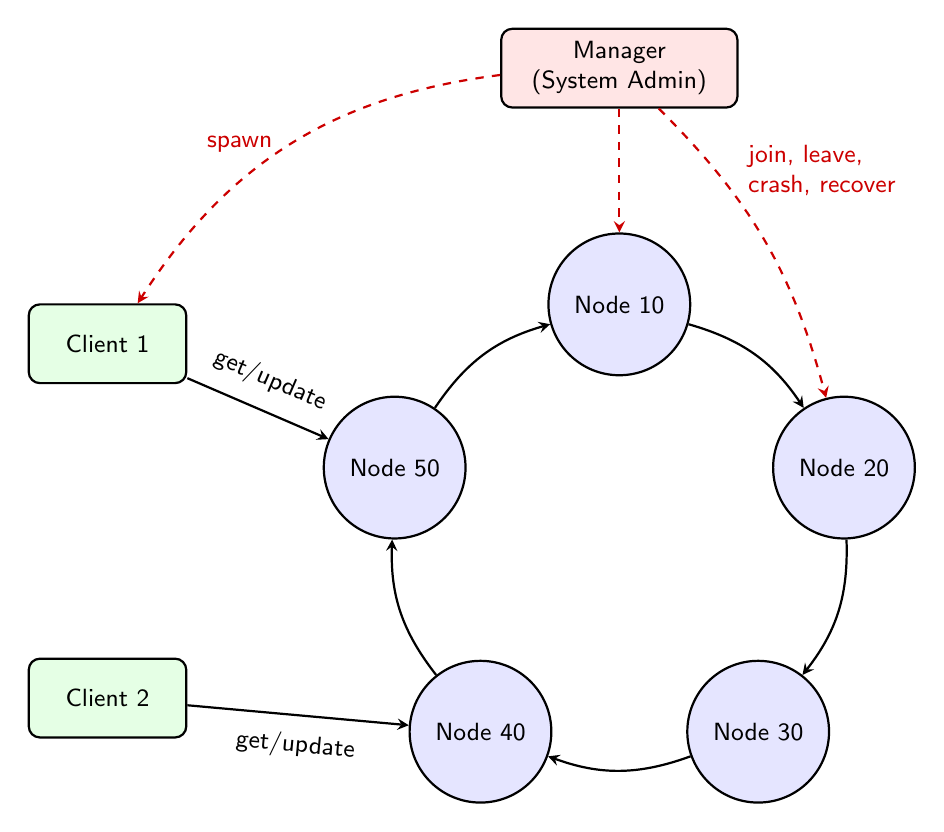
\begin{tikzpicture}[
        node distance=2cm,
        every node/.style={font=\sffamily\small},
        actor/.style={circle, draw=black, thick, fill=blue!10, minimum size=1.8cm, align=center},
        manager/.style={rectangle, draw=black, thick, fill=red!10, rounded corners, minimum width=3cm, minimum height=1cm, align=center},
        client/.style={rectangle, draw=black, thick, fill=green!10, rounded corners, minimum width=2cm, minimum height=1cm, align=center},
        arrow/.style={thick, ->, >=stealth},
        dashed_arrow/.style={thick, dashed, ->, >=stealth, color=red!80!black}
        ]

        % The Ring of Nodes
        \def\radius{3cm}
        \node[actor] (N10) at (90:\radius) {Node 10};
        \node[actor] (N20) at (18:\radius) {Node 20};
        \node[actor] (N30) at (306:\radius) {Node 30};
        \node[actor] (N40) at (234:\radius) {Node 40};
        \node[actor] (N50) at (162:\radius) {Node 50};

        % Ring connections (clockwise)
        \draw[arrow] (N10) to[bend left=20] (N20);
        \draw[arrow] (N20) to[bend left=20] (N30);
        \draw[arrow] (N30) to[bend left=20] (N40);
        \draw[arrow] (N40) to[bend left=20] (N50);
        \draw[arrow] (N50) to[bend left=20] (N10);

        % Manager Entity
        \node[manager] (Manager) at (0, 6) {Manager\\(System Admin)};

        % Client Entities (Moved further left to stretch the arrows)
        \node[client] (C1) at (-6.5, 2.5) {Client 1};
        \node[client] (C2) at (-6.5, -2) {Client 2};

        % Manager to Node interactions (dashed red arrows)
        \draw[dashed_arrow] (Manager) -- node[right=40, align=left, xshift=0.1cm] {join, leave,\\crash, recover} (N10);
        \draw[dashed_arrow] (Manager) to[bend left=15] (N20);

        % Manager to Client interactions
        \draw[dashed_arrow] (Manager) to[bend right=25] node[left, xshift=-0.1cm] {spawn} (C1);

        % Client interactions (solid black arrows)
        % Added 'above=0.1cm' and 'below=0.1cm' to lift the text off the line
        \draw[arrow] (C1) -- node[above=0.1cm, sloped] {get/update} (N50);
        \draw[arrow] (C2) -- node[below=0.1cm, sloped] {get/update} (N40);

    \end{tikzpicture}
\end{figure}
